\documentclass[a4paper,10pt]{scrartcl}

\usepackage[utf8]{inputenc}
\usepackage[ngerman]{babel}
\usepackage[T1]{fontenc}
\usepackage{amsmath}
\usepackage{graphicx}
\usepackage{hyperref}
\usepackage{eso-pic} 
\usepackage{mathtools}

\newcommand\BackgroundPic{% 
   \put(0,0){% 
      \parbox[b][\paperheight]{\paperwidth}{% 
         \vfill 
         \centering{
\includegraphics{images/videoChop.png}} 
         \vfill 
      } 
   } 
} 

\title{Medienprojekt I \\ Thema: Videochop}
\author{Michael Duve, Felix Maulwurf, Angelina Staeck}
\date{13.01.2014}
\begin{document}
\maketitle
\newpage
\AddToShipoutPicture{\BackgroundPic}
\tableofcontents
\newpage
\section{Projektteilnehmer}
\subsection{Michael Duve}
\begin{center}

\includegraphics[height=90px, width=90px]{images/micha.jpg}\\
\textbf{Medieninformatik Fachsemester 4} \\
\vspace*{1.5mm} 
HTML5, CSS3, JS, PHP, MySQL, Webapps iOS,\\
Grundkenntnisse Server,
Java, min. Python
Photoshop, Illustrator, InDesign
Repositories (Git, Mercurial), JIRA, Documentation
\end{center}
\subsection{Felix Maulwurf}
\begin{center}

\includegraphics[height=90px, width=90px]{images/felix.jpg}\\
\textbf{Medieninformatik Fachsemester 4} \\
\vspace*{1.5mm} 
HTML5, CSS3, JS, PHP, MySQL, Java,\\
Photoshop, Illustrator, After Effects,
3DSMax,\\
Cinema4D, Office, Repositories (Git), LaTeX
\end{center}
\subsection{Angelina Staeck}
\begin{center}

\includegraphics[height=90px, width=90px]{images/angi.jpg}\\
\textbf{Medieninformatik Fachsemester 4} \\
\vspace*{1.5mm} 
HTML5, CSS3, JS, PHP, \\
Java, SQL, Illustrator, Photoshop
\end{center}
\newpage
\section{Projektbeschreibung}
VideoChop ist eine Webanwendung basierend auf JavaScript, die dem Anwender  ein einfaches und intuitives „Videoschnittstudio“ zur Verfügung stellt. VideoChop soll es ermöglichen Videos vom Desktop direkt in den Browser zu ziehen. Es steht dem User frei, ob er ein oder mehrere Videos schneiden oder zusammenfügen möchte. VideoChop wird eine übersichtliche und schlichte Oberfläche bieten, die auch Anfänger nicht überfordert. Die Videos werden in einer Zeitleiste organisiert und beschnitten. Wer mal eben schnell ein Video schneiden will, um Vor- oder Abspann oder etwaige Längen zu entfernen, braucht keine Speicher fressende und kompliziert zu bedienende Videobearbeitung. Der Nutzer kann sich sein Werk vor dem Abspeichern im Browser als Vorschau ansehen.
\subsection{Idee}
Die Idee ist es, dass VideoChop dem Nutzer eine Plattform zur Verfügung stellt, die keinerlei Daten serverbasiert speichert. Das Projekt basiert auf JavaScript und nutzt somit die Rechenressourcen des Nutzers. Die Belastung für den Server sind damit minimal. VideoChop soll einfach, intuitiv und schnell sein. JavaScript ist sehr mächtig, allerdings sind zu Projektbeginn die Möglichkeiten und Umsetzbarkeiten noch nicht geklärt.
\subsection{Zukunft}
Zukünftig sollen weitere Funktionalitäten hinzukommen. 
\begin{itemize}
    \item Handlebars benutzen
    \item Ordner/Gruppierungen der Videos
    \item Frames pro Sekunde anzeigen
    \item Mute-Button für einzelne Videos
    \item Eigene Audiospur einbaubar
    \item Text auf Video ablegen
    \item Import unterschiedlicher Formate
	\item Export in verschiedene Formate
	\end{itemize}
\subsection{Probleme}
\begin{itemize}
	\item Keine! Lediglich die Zeit fehlt ;)
	\end{itemize}
\subsection{Was läuft gut?}
Das zusammensetzen klappt mittlerweile gut. Wir haben große Fortschritte gemacht. Das neue Design gefällt uns Dreien.
\subsection{Was läuft nicht so gut?}
Das Fertigstellen einer Version 1.0 zögert sich immer wieder hinaus, weil Fehler gefunden werden. Mit 3 Personen ist das Projekt echt sehr umfangreich.
\subsection{Teamstruktur und Aufteilung?}
Es macht immer noch jeder alles. Meist teilen wir uns die Tickets selber zu
\subsection{Was ist noch offen?}
\begin{itemize}
    \item VideoExporter - Modul noch nicht angelegt, test-case ist fertig
    \item FAQ Seite soll noch eingerichtet werden
    \item Help-Screen - Anzeige direkt beim start
    \item New project button noch nicht funktional
    \item VideoTimeline - testcase ist halb fertig, Modul muss noch angelegt werden
    \item Videopreview - Modul angefangen aber unvollständig, testcase angefangen
    \item Import unterschiedlicher Formate
	\item Export in verschiedene Formate
	\end{itemize}
\section{Layout}
Komplett neues Design: Das kostete uns am meisten Zeit\\
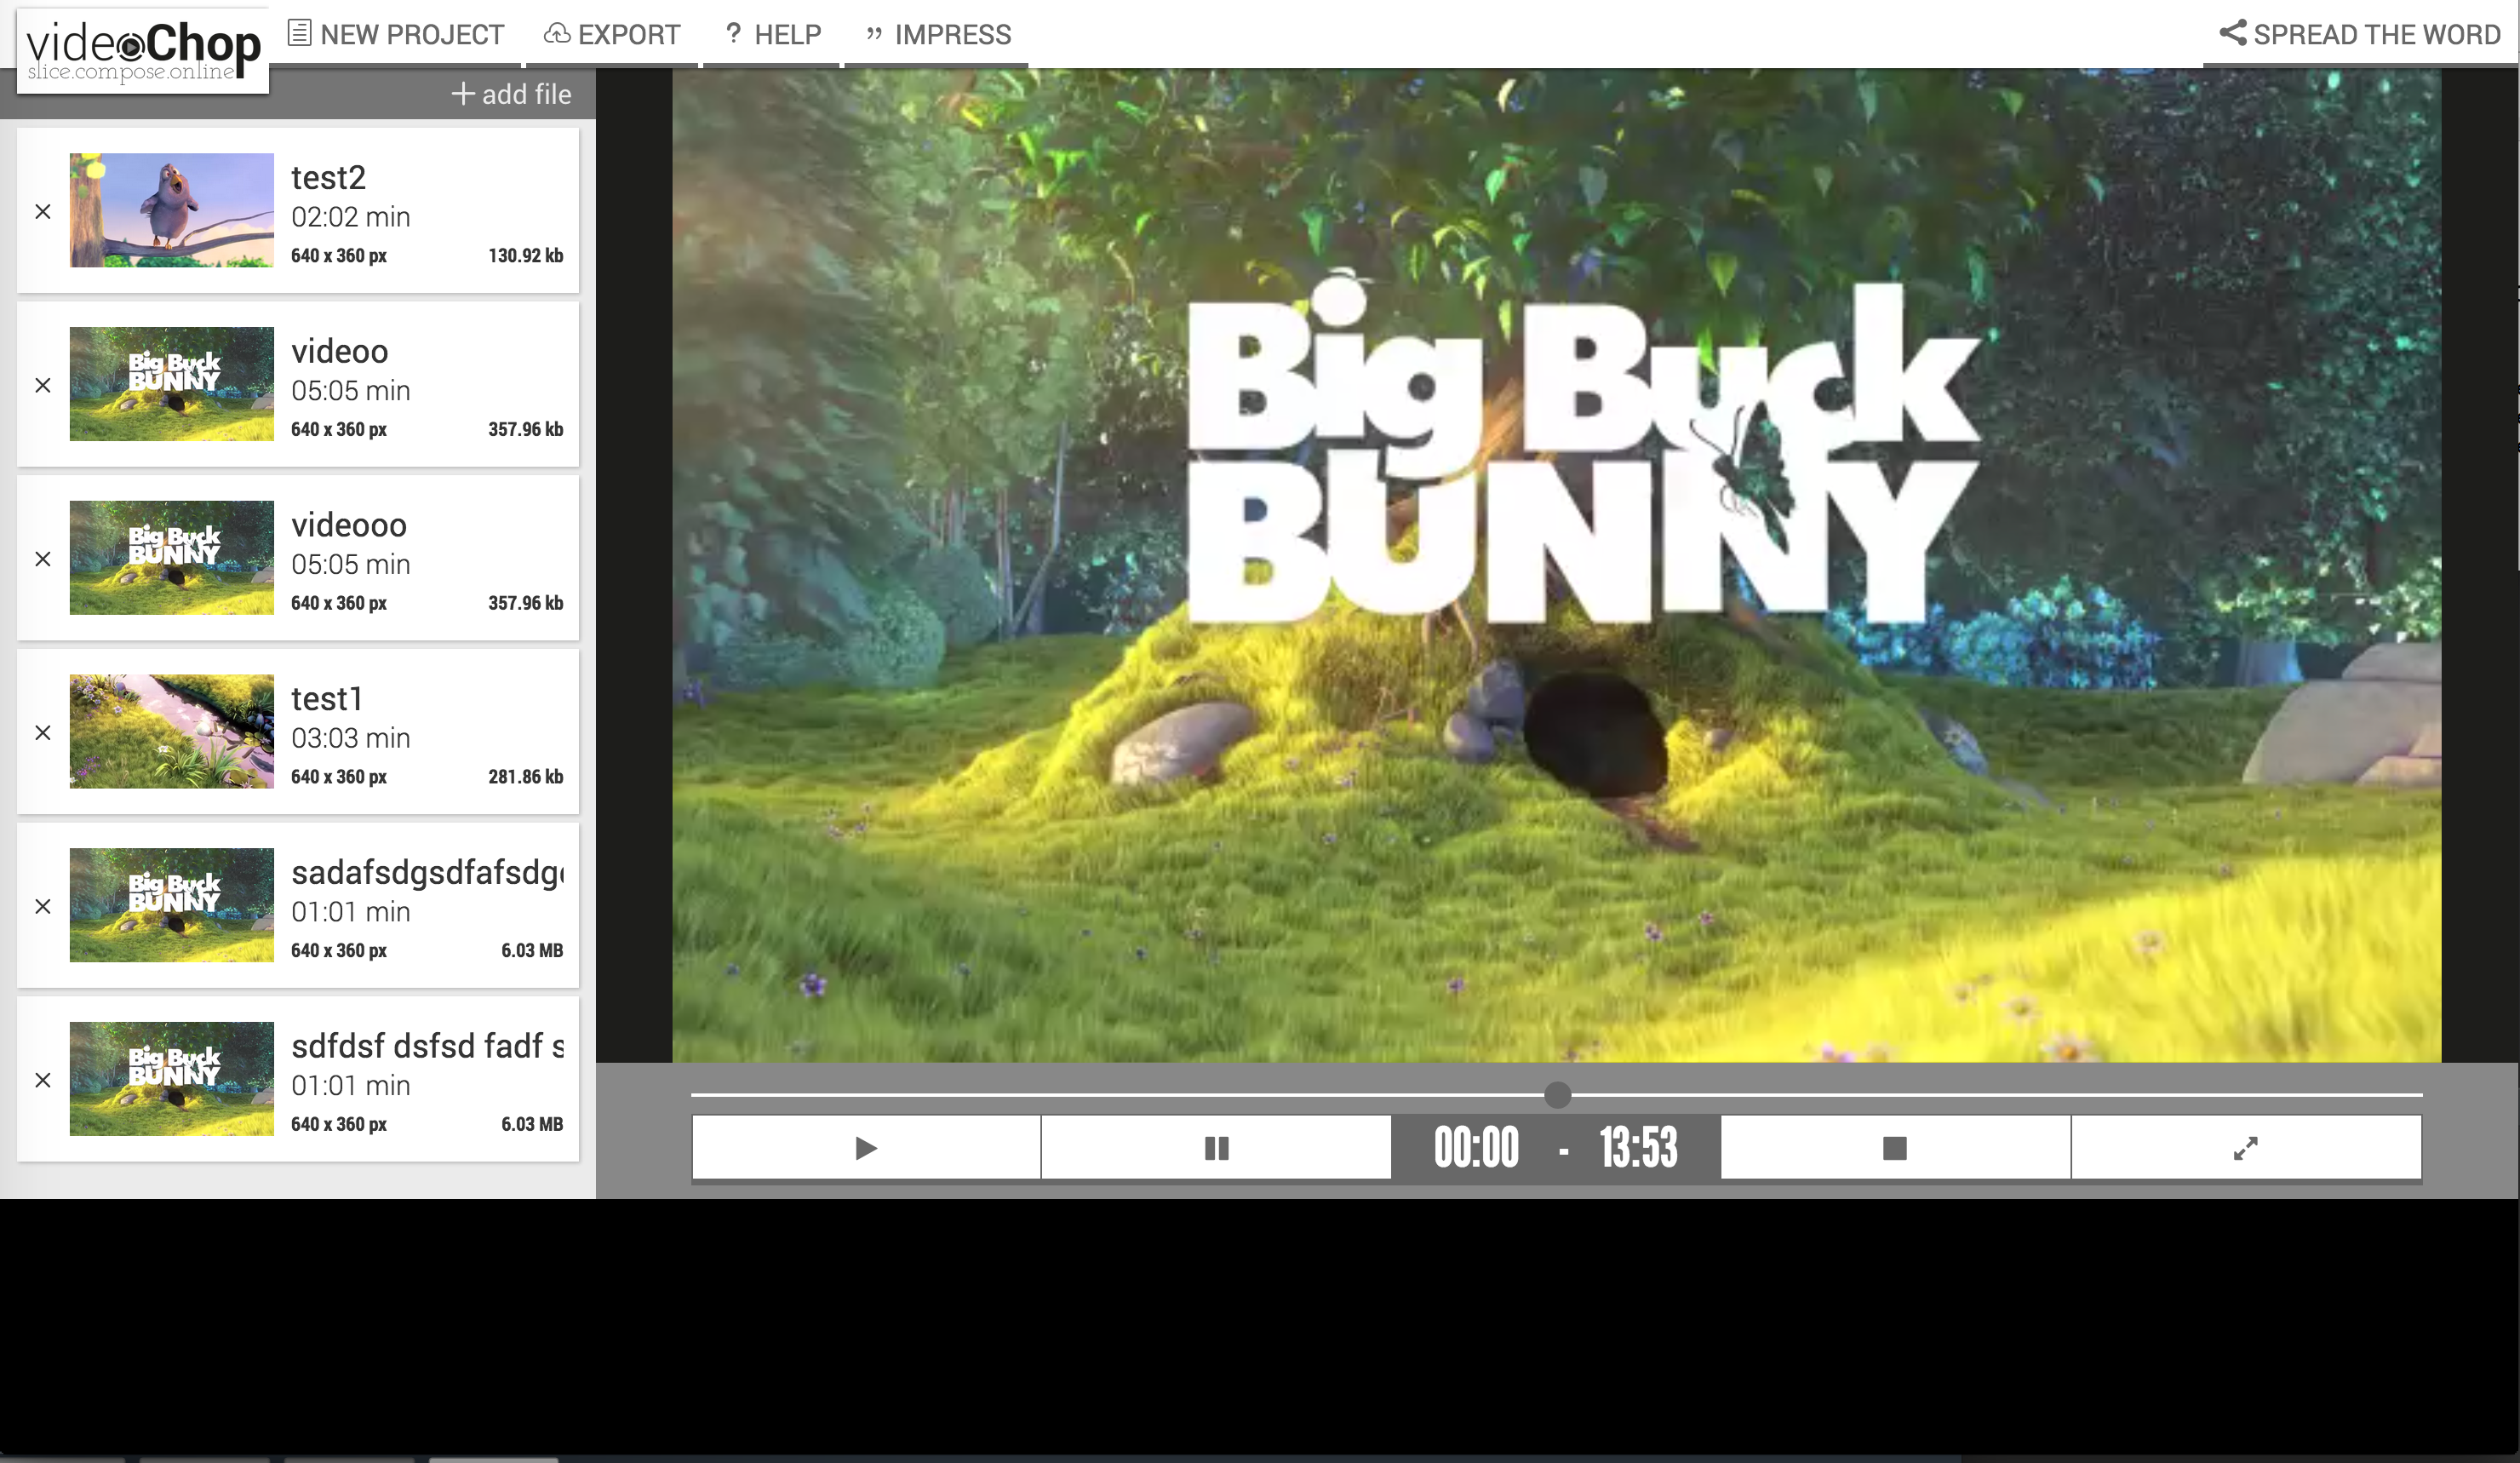
\includegraphics[width=400px]{images/layout.png}\\
\newpage
\section{Testcases}
Für jede Funktion haben wir Testcases erstellt. Die Testcases werden jeweils nach Bedarf erweitert. Das bedeutet, dass im weiteren Verlauf der Entwicklung neue Testcases hinzukommen können. Die Testcases sind spezifisch und nicht modular programmiert. Aus den Testcases haben wir unsere Module abgeleitet.
\subsection{Drag-Drop}
\textbf{http://localhost/videochop/testcases/drag-drop-updated/index.html} \\
Der Drag and Drop Testcase dient als Grundlage für die spätere Timeline.\\
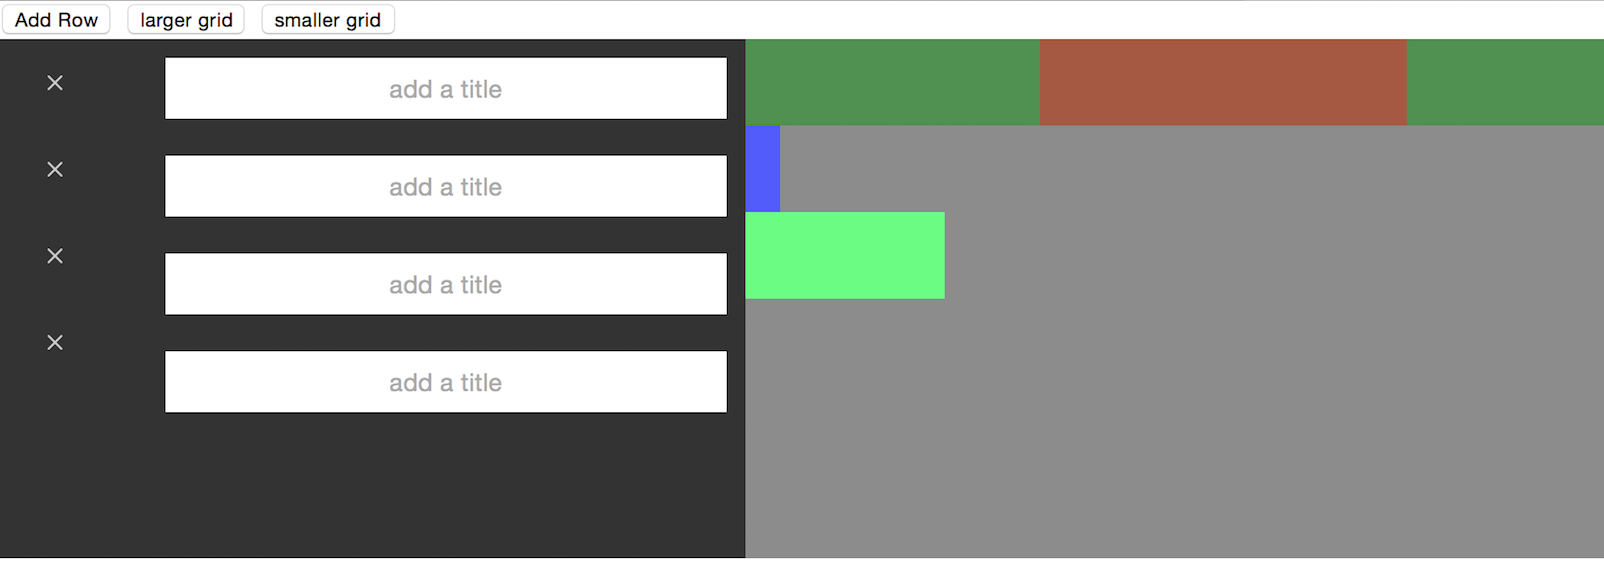
\includegraphics[height=176px, width=300px]{images/draganddrop.png}\\
Der Testcase wurde angepasst. Der vorherige Test-Case verursachte zu viel Inkosistenz beim Hinzufügen und Löschen.
\subsection{FFMPEG}
\textbf{testcases - ffmpeg - index.html} \\
FFmpeg funktioniert nun einwandfrei und wird im nächsten Milestone als Modul implementiert. Der Name des Moduls ist VideoExporter
\newpage
\section{Module}
\subsection{Video Item}
\textbf{testcases - module\_video\_item - index.html} \\
\textbf{videochop - js - modules - videoItem.js} \\
Jedes vom Nutzer in den Browser gezogene Video wird duch ein VideoItem repräsentiert. Es speichert alle relevanten Daten. Die Daten werden beim in den Browser ziehen vom Modul VideoItemLoader ausgelesen und in ein neues VideoItem geschrieben.\\
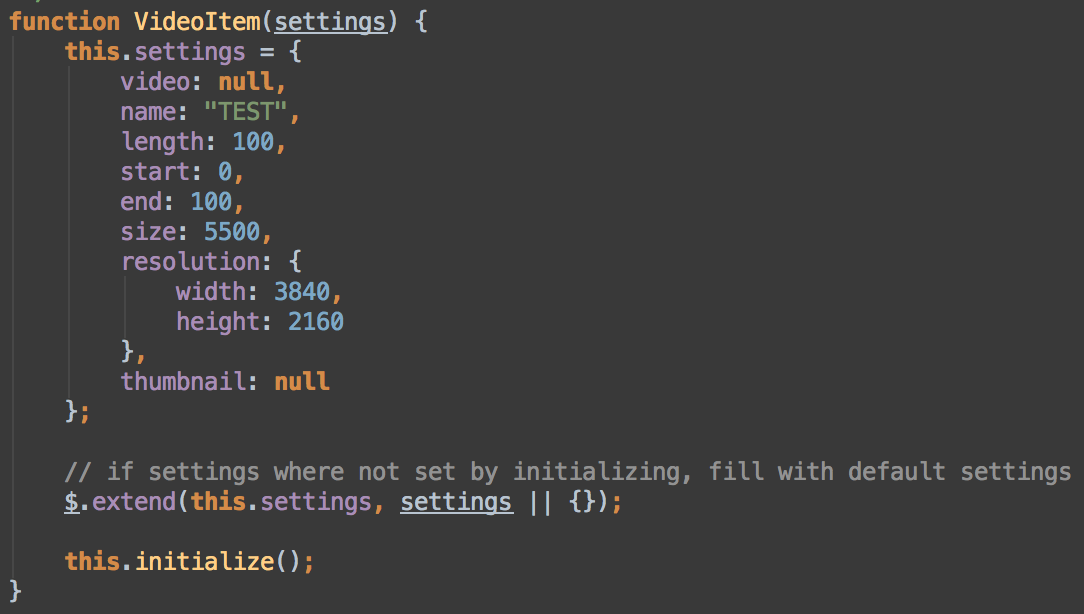
\includegraphics[height=176px, width=375px]{images/videoitem.png}\\
Das VideoItem-Modul brauchte noch weitere Settings und Anpassungen. Einmal muss es das geladene Video halten. Die URL war als base64-String zu groß für das DOM, sobald zu viele Videos auf der Seite verbaut waren. Wir haben das Problem durch Veränderung der VideoURL und der Thumbnail-URL mittels Object-URL umgangen \\
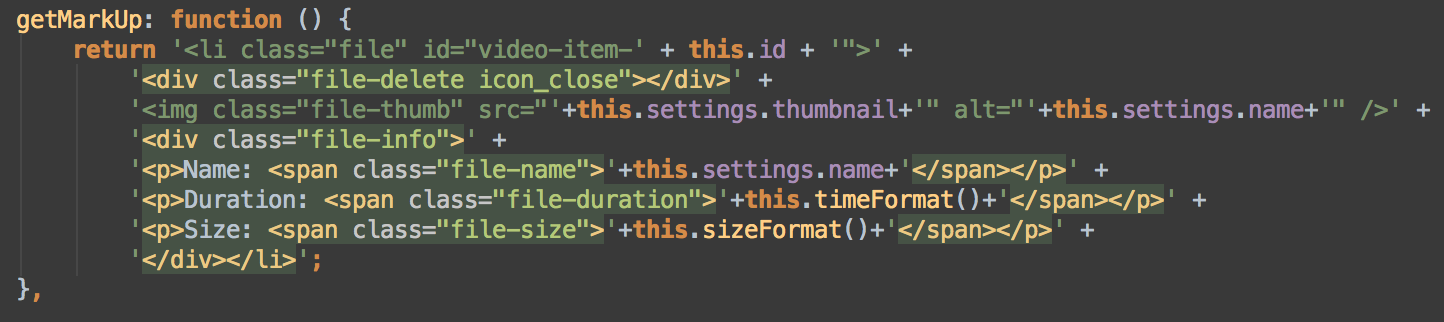
\includegraphics[height=120px, width=375px]{images/videoitem2.png}\\
\subsection{Video Item Loader}
\textbf{testcases - module\_video\_item\_loader - index.html} \\
\textbf{videochop - js - modules - videoItemLoader.js} \\
Hier mussten wir auch ein paar kleinere Anpassungen machen. Dadurch, dass die duration eines Videos erst nach dem Event "metadataloaded" zurückgegeben wird, mussten wir auf das asynchrone Event warten und dann erst das Video zur List hinzufügen.
\subsection{Video List}
\textbf{testcases - module\_video\_list - index.html} \\
\textbf{videochop - js - modules - videoList.js} \\
Hier waren auch Anpassungen notwendig. Wir wollten das man sich die Items in der VideoList anordnen kann wie man möchte. Das funktioniert nun. Zusätzlich wurde VideoList nun auch in unseren Controller eingebaut und funktioniert super mit dem neuen Layout.\\
\subsection{Video Preview}
Das Modul wurde angelegt. Es iteriert über eine Liste von VideoItems und spielt das gerade aktive Video von videoItem.settings.start bis zum vorgegebenen Ende ab. Dann Wechselt das Video zum nächsten. Momentan ist unser Gedanke die HTML-Videos aus und einzublenden, da das Wechseln der URL zu lange brauchen würde.
\subsection{Video Controls}
Dieses Modul brauchen wir so nicht mehr. VideoPreview übernimmt die Aufgaben.
\subsection{Video Timeline}
Dadurch, dass wir den Testcase Drag and Drop noch mal geupdatet haben, konnten wir dieses Modul nicht anfangen. Zum nächsten MS wird es aber angefangen sein.
\section{Zeitaufwand}
\begin{tabular}{|c|c|c|}\hline
	\textbf{Aufgabe} & \textbf{Zeitaufwand} \\ \hline
	
	Design-/Layoutkonzept & 5,5 Stunden \\ \hline
	
	repsponsive Layoutumsetzung & 16 Stunden \\ \hline
	
	Testcase Drag and Drop & 5 Stunden mit Recherche \\ \hline
	
	PreviewVideo & 7 Stunden \\ \hline
	
	Anpassungen alter Module & 5 Stunden \\ \hline

	Reparatur Logo & 1 Stunde \\ \hline
	
	Sammlung FAQ-Fragen & 0,5 Stunden \\ \hline
	
	GIT-Comments und Aufräumen & 0,5 Stunden \\ \hline

	Bericht & 1,5 Stunden \\ \hline

	Debugging & 3 Stunden \\ \hline
	
	SCSS-Refactoring & 1 Stunden \\ \hline

	Insgesamt & 56 Stunden \\ \hline

	
 \end{tabular}
 \newpage
\section{Externe Plugins}
\subsection{jQuery UI}
URL: http://jqueryui.com\\
DOM-Elemente sind interaktiv nutzbar
\subsection{jQuery Collision}
URL: http://eruciform.com/static/jquidragcollide/jquery-ui-draggable-collision.js\\
Wird benutzt, damit zwei VideoItems in der Timeline nicht aufeinander liegen dürfen
\subsection{FFMPEG}
URL: https://github.com/bgrins/videoconverter.js\\
Wird benutzt um Videos umwandeln zu können.
\subsection{Popcorn JS Capture}
URL: https://github.com/rwaldron/popcorn.capture\\
Wird benutzt, um ein Poster von einem Video an einer beliebigen Position als Thumbnail zu extrahieren
\subsection{Filereader}
URL: https://github.com/bgrins/filereader.js/\\
Ein Plugin, die den Umgang mit Drag \& Drop von Dateien STARK vereinfacht
\subsection{UserAgent Parser}
URL: https://github.com/faisalman/ua-parser-js\\
Wird benutzt um festzustellen mit welchem Browser der User unterwegs ist
\subsection{FileSaver}
URL: https://github.com/eligrey/FileSaver.js\\
Hiermit können wir Dateien direkt auf dem Desktop des Users speichern, weil dieses Plugin die HTML5-Api ausbessert
\subsection{jQuery, Modernizr \& Require}
Dazu brauchen wir keine Beschreibung.
\end{document}